%\documentclass[preprint,3p,times,twocolumn]{elsarticleUS}
\documentclass[review,3p,times]{elsarticleUS}
\usepackage{amssymb}
\usepackage{amsmath}
\usepackage{graphicx}
\usepackage{bm}
\usepackage{yhmath}
\usepackage{subfigure}
\usepackage{multirow}
\usepackage{color}
\usepackage{xcolor}
\usepackage{subdepth}
\usepackage[nomarkers,lists]{endfloat}

\def\pp#1#2{\frac{\partial #1}{\partial #2}}

\biboptions{comma,sort&compress}

\journal{Combustion and Flame}

\makeatletter
\def\@author#1{\g@addto@macro\elsauthors{\normalsize%
    \def\baselinestretch{1}%
    \upshape\authorsep#1\unskip\textsuperscript{%
      \ifx\@fnmark\@empty\else\unskip\sep\@fnmark\let\sep=,\fi
      \ifx\@corref\@empty\else\unskip\sep\@corref\let\sep=,\fi
      }%
    \def\authorsep{\unskip,\space}%
    \global\let\@fnmark\@empty
    \global\let\@corref\@empty  %% Added
    \global\let\sep\@empty}%
    \@eadauthor={#1}
}
\makeatother

\begin{document}

\begin{frontmatter}

\title{NTC-affected ignition and low-temperature flames in nonpremixed DME/air counterflow}

\author[Princeton]{Sili~Deng}
\author[Princeton]{Peng~Zhao}
\author[Princeton]{Delin~Zhu}
\author[Princeton,Tsinghua]{Chung K.~Law\corref{cor}}
\cortext[cor]{Corresponding Author: cklaw@princeton.edu}

\address[Princeton]{Department of Mechanical and Aerospace Engineering, Princeton University, Princeton, NJ 08544, USA}
\address[Tsinghua]{Center for Combustion Energy, Tsinghua University, Beijing 100084, China}

\begin{abstract}
An experimental study, supported by computation, was conducted on the coupling of NTC-chemistry and transport in the low-temperature ignition and the associated steady burning in nonpremixed DME/air counterflow.  In particular, the presence of low-temperature chemical reactivity was detected nonintrusively by using a photomultiplier tube combined with a filter to capture the chemiluminescence of HCHO, which is a characteristic intermediate species formed in low-temperature chemistry.  Furthermore, the ignition temperature was determined through high-sensitivity infrared imaging with proper discrimination of the background signal. Experimental results show that the transport-coupled low-temperature, NTC chemical reactivity is enhanced with smaller strain rate, higher air boundary temperature, and is insensitive to the fuel concentration.  These findings agree well with those obtained from computation using detailed chemistry, leading to further identification of the controlling chemistry.
\end{abstract}

\begin{keyword} 
Negative Temperature Coefficient (NTC) \sep Dimethyl Ether (DME) \sep
Nonpremixed Counterflow \sep Low-temperature Chemistry \sep Chemiluminescence
\end{keyword}

\end{frontmatter}

%\clearpage % For word count
\section{Introduction}

Negative temperature coefficient (NTC) refers to the phenomenon that the ignition delay time of a hydrocarbon/air mixture increases with increasing initial temperature within a certain low- to intermediate-temperature range in relation to its adiabatic flame temperature.  This range is typically between $600$ and $800$ K at $1$ atm.  This phenomenon has been extensively studied since it is essential to the combustion of many hydrocarbon fuels, especially for processes associated with engine knock. However, most of these studies and the understanding gained therein are based on homogenous systems, such as those employing shock tubes~\cite{ciezki93}, flow reactors~\cite{wada11}, jet stirred reactors~\cite{veloo13}, and rapid compression machines~\cite{mittal08}.  Since nonuniformities invariably exist in practical combustion systems, the coupling between the NTC chemistry and convective-diffusive transport processes needs to be considered.  It is reasonable to expect that in a chemically reacting flow, when the characteristic transport time becomes comparable to that of the NTC chemical time, the two processes will be strongly coupled to affect the local response.  By the same reasoning, when the characteristic residence time becomes relatively long, the NTC chemistry will be decoupled from the transport processes and the system response will recover to that of the homogeneous mixture.  Indeed, recently Law and Zhao~\cite{law12} and Zhao and Law~\cite{zhao13} have computationally identified the presence of distinctive NTC-affected chemical reactivity and an associated weakly burning flame in the steady counterflow system, showing the existence of a secondary ignition-extinction S-curve grafted onto the lower branch of the primary S-curve. Furthermore this secondary S-curve becomes more pronounced at lower strain rates and higher pressures.

The primary objective of the present investigation is to experimentally explore if the computationally predicted subject phenomenon indeed exists, and to characterize its response if the exploration is affirmative.  The investigation is a challenging one because of the weak reactivity and the correspondingly weak exothermicity involved.

Dimethyl ether (DME) was selected as the fuel for the present study because it is gaseous and is one of the simplest hydrocarbons exhibiting the NTC behavior.  Furthermore, detailed reaction mechanisms for low- and high-temperature DME oxidation~\cite{curran98,fischer00,curran00,zhao08} have been developed and validated for burner stabilized flames~\cite{kaiser00}, nonpremixed counterflow flame ignition~\cite{zheng05}, laminar flame speeds~\cite{qin05}, and studies using rapid compression machines~\cite{mittal08}.  This allows the computational simulation and thereby guidance and verification of the experimentation with moderate confidence. In particular, the present computation was conducted using a skeletal mechanism of $39$ species~\cite{bansal11} reduced from the detailed mechanism of Zhao \emph{et al.}~\cite{zhao08}.

In the following, we shall systematically present the experimental and numerical identification of the NTC-affected ignition and the associated low-temperature flame in the nonpremixed counterflow.  A conference version of the present work was presented in~\cite{deng13}.

\section{Experimental Investigation}

A schematic of the experimental setup is shown in Fig.~\ref{fig:setup}; detailed descriptions of the counterflow experimental apparatus are given in~\cite{fotache95,liu10a}.  Briefly, the apparatus consists of two vertically oriented opposing quartz nozzles with diameters of $20$ mm and separated by $20$ mm.  A heated air or N$_2$ stream is issued from the upper nozzle and impinges against a room-temperature N$_2$-diluted DME steam issued from the lower nozzle.  Both upper and lower streams are shielded by coflowing N$_2$ to minimize disturbance from the environment.  In a typical counterflow ignition experiment, ignition is achieved by gradually increasing the air boundary temperature until a visible flame appears. The exit temperature, measured by a thermocouple with radiation correction~\cite{zheng06}, is then defined as the ignition temperature. Single-point laser Doppler velocimetry (LDV) is used to measure the axial flow velocity along the centerline to determine the local strain rate of the flow.

While the above procedure has been successfully used in previous studies of ignition and the diagnosis of the resulting flame for strongly burning flames, for which the instant of ignition can be observed visually, no bright flame or visually-detectable reaction front could be observed for the present NTC-affected ignition within the temperature range of interests ($600$-$800$ K).  Furthermore, no discernable heat release was detected by using a thermocouple, ostensibly due to the small amount of heat release from the low-temperature chemistry.  In the absence of a flame, it was also not clear the extent of the disturbance introduced by the thermocouple to the flow field as well as the ignition kernel.

In view of the above limitations, we have resorted to optical detection and measurement. A photomultiplier tube (PMT) was subsequently applied to detect any NTC-related chemiluminescence, noting that experimental studies in homogeneous systems have shown that the NTC-induced chemistry have characteristic chemiluminescence spectra, with a small amount of heat release~\cite{sheinson73,ohta91}.  These studies further showed that a large amount of formaldehyde (HCHO) is formed from the low-temperature chemistry and the pale blue chemiluminescence from HCHO characterizes the associated low-temperature reaction~\cite{gaydonbook}.  Based on these characteristics, we designed our experiment as shown in Fig.~\ref{fig:setup}. Here a Hamamatsu 931B PMT combined with focusing lens system and a Newport filter (10BPF10-400) was used to detect the chemiluminescence corresponding to the characteristic wavelength of formaldehyde (peaks around $400$ nm) and to reduce noise light signals from the counterflow chamber. The PMT signal was then collected and processed with a SR510 lock-in amplifier to further diminish the noise.  Results based on this experimentation to demonstrate the existence of the low-temperature chemistry in the counterflow are discussed in Sec.~\ref{sec:4.1}.  This is followed by an investigation based on infrared imaging to identify the state of ignition, in Sec.~\ref{sec:4.2}. 

\begin{figure}[t]
  \centering
  \scriptsize
%  \vspace{-0.1in}
  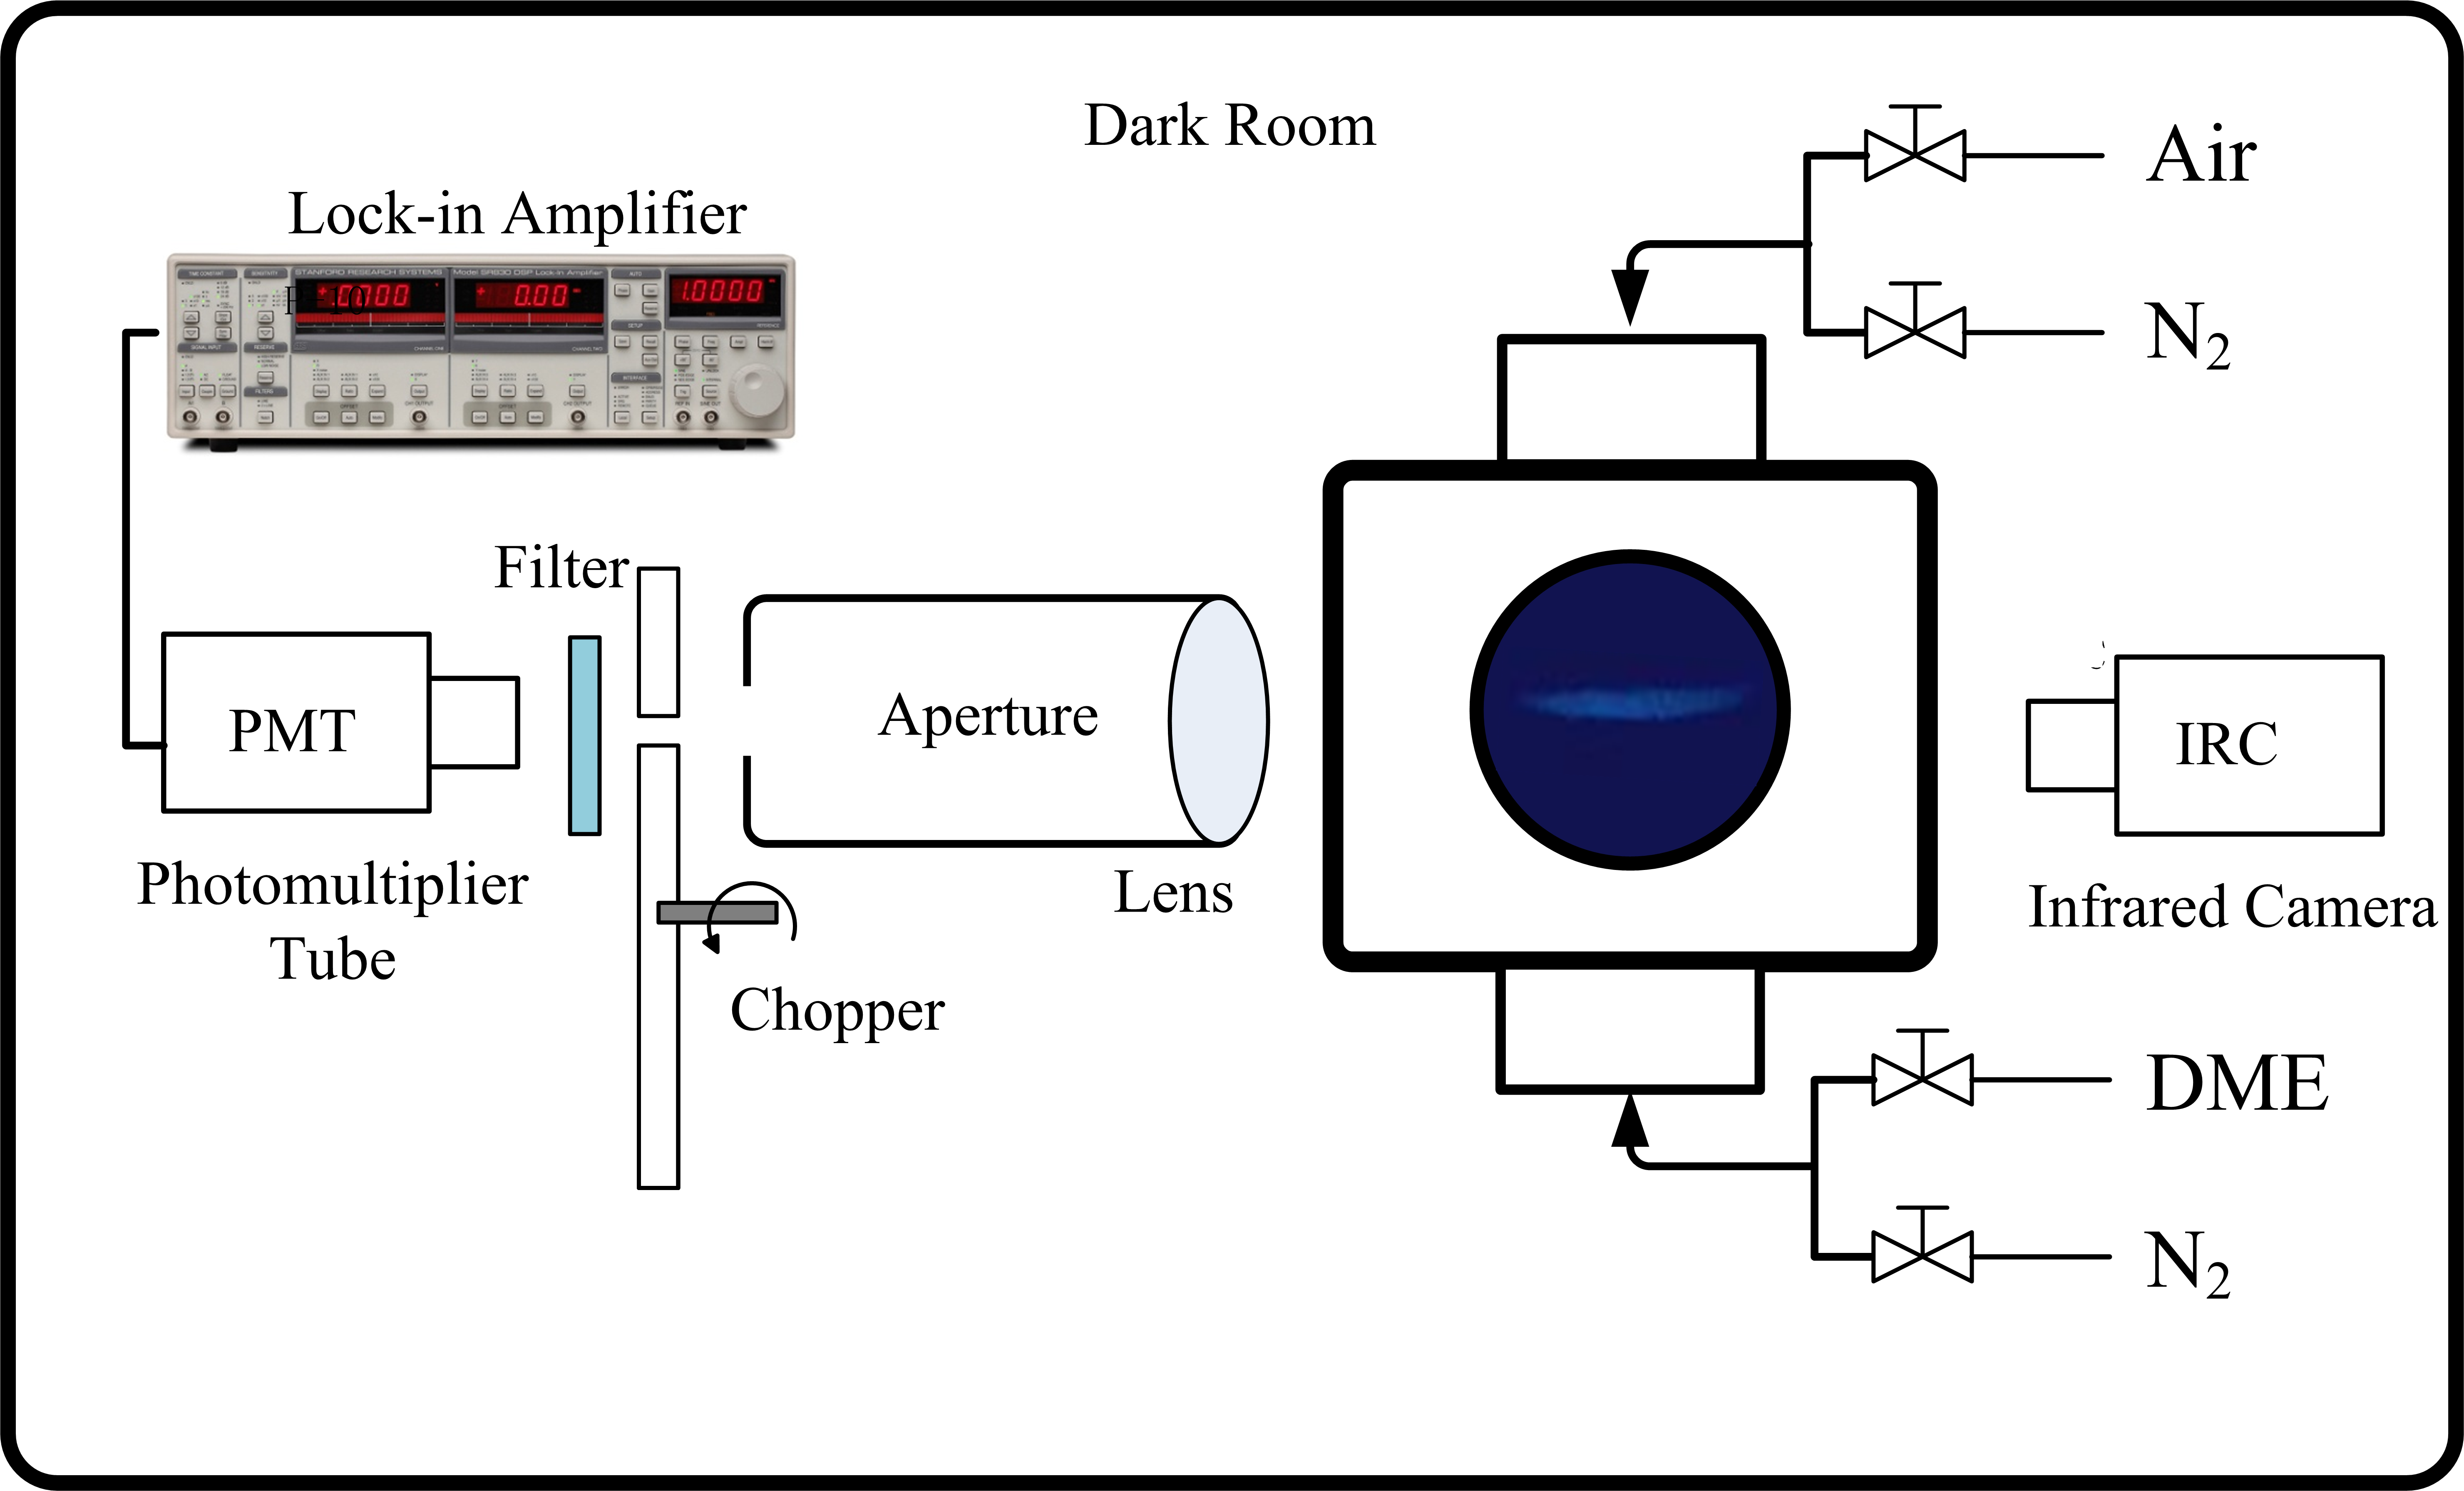
\includegraphics[width=0.8\textwidth]{Experimental_Setup.png}
  \normalsize
%  \vspace{-0.1in}
  \caption{Schematic of the experimental system.}
  \label{fig:setup}
\end{figure}

\section{Computational Investigation}

The steady-state response of a one-dimensional reactive system subjected to heat loss can be studied via the S-curve analysis~\cite{lawbook}. In such an analysis, a system response such as the maximum temperature or radical concentration is monitored for variations of an imposed parameter such as the air temperature, for a given strain rate of the flow, or the system Damk\"ohler number.  For a global one-step overall reaction with large activation energy, the intrinsically nonlinear Arrhenius kinetics frequently yields multiple solutions characterized by an S-shaped response curve, with the lower and upper turning points respectively designate the ignition and extinction states of the system.  Such triple-branch S-curves also frequently emerge for simulations using detailed reaction mechanisms, while more complex response curves with additional turning points have also been obtained, for example for hydrogen oxidation~\cite{kreutz94,fotache98} and methane oxidation~\cite{liu09}. 

The governing equations for the counterflow nonpremixed flame are presented in Giovangigli \emph{et al.}~\cite{giovangigli87}. The numerical code adopted to solve them~\cite{smooke86} employs the damped Newton method and time integration solution scheme, with boundary conditions specified on both sides of the potential flow.  The S-curve marching is performed using the flame-controlling method of Nishioka \emph{et al.}~\cite{nishioka96} with detailed chemistry~\cite{kee89} and transport database~\cite{kee83}.

The critical state of ignition is assessed through the lower turning point of the S-curve.  The simulation conditions are as follows: the fuel-side mixture consists of DME and nitrogen with a fixed temperature of $300$ K, and the oxidizer side is standard air at a high temperature.  The separation distance between the two nozzle exits is $20$ mm, with the origin being fixed at the fuel exit.  To generate an S-curve, marching is performed by either changing the air-side boundary temperature with fixed strain rate or equivalently the strain rate with fixed air-side boundary temperature.  Following Law and Zhao~\cite{law12} and Zhao and Law~\cite{zhao13}, the distinct turning points of the NTC S-curves of DME are captured, and the calculated ignition temperature at different strain rates as well as different boundary fuel concentrations are compared with the experimental results.

\section{Results and Discussion}
\subsection{Identification of the low-temperature, NTC, flame} \label{sec:4.1}

Validation results for the experimental system are shown in Fig.~\ref{fig:M}.  Specifically, when the PMT captures the photons corresponding to the characteristic wavelength of HCHO (peaks around $400$ nm), it outputs negative impulses to the oscilloscope, with the amplitudes of these impulses represent the light intensity.  Figure~\ref{fig:M} shows that such signal intensity drops after replacing either N$_2$-diluted DME with pure N$_2$ issued from the lower nozzle (at point a), or air with N$_2$ issued from the upper nozzle (at point c), hence demonstrating that the signal is due to the simultaneous presence of air and DME.  Since replacing air with the same flow rate of N$_2$ barely affects the temperature profile and the flow field, the signal difference between the air/DME and N$_2$/DME cases indicates the existence of NTC chemical activities.  It is noted that the signal from N$_2$/DME thermal pyrolysis is minimal in the present study, such that the difference in the chemically reactive and non-reactive cases can be completely attributed to the low-temperature oxidation chemistry.  


\begin{figure}[t]
  \centering
  \scriptsize
  \vspace{-0.1in}
  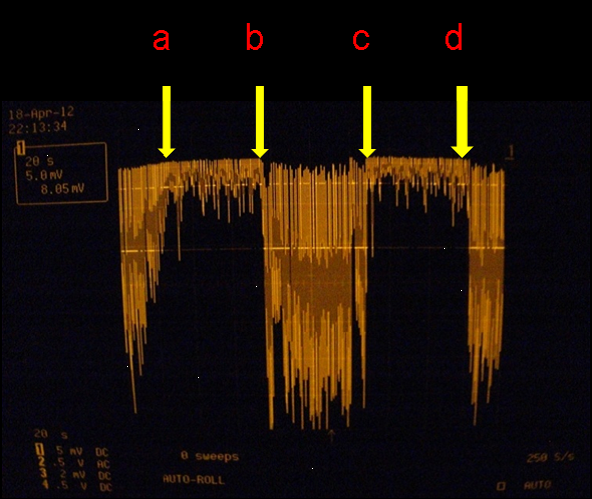
\includegraphics[width=0.5\textwidth]{M.png}
  \normalsize
%  \vspace{-0.1in}
  \caption{"M" shaped signal. a.~Switch Air/DME to Air/N$_2$; b.~Switch Air/N$_2$ to Air/DME; c.~Switch Air/DME to N$_2$/DME; d.~Switch N$_2$/DME to Air/DME.}
  \label{fig:M}
\end{figure}

In Fig.~\ref{fig:PMT}, the chemiluminescence intensity from the HCHO under the strain rates of $40$, $60$, and $100$ /s were measured as a function of the air boundary temperature.  The time-averaged signal were acquired by the lock-in amplifier with an integration time of three seconds to minimize the noise, and the error bars show the standard deviation of the signals based on $1000$ samplings. The results clearly show that the low-temperature chemistry becomes more pronounced at higher air temperatures and lower strain rates, with more HCHO produced and therefore stronger chemiluminescence from it.

\begin{figure}[t]
  \centering
  \scriptsize
  \vspace{-0.1in}
  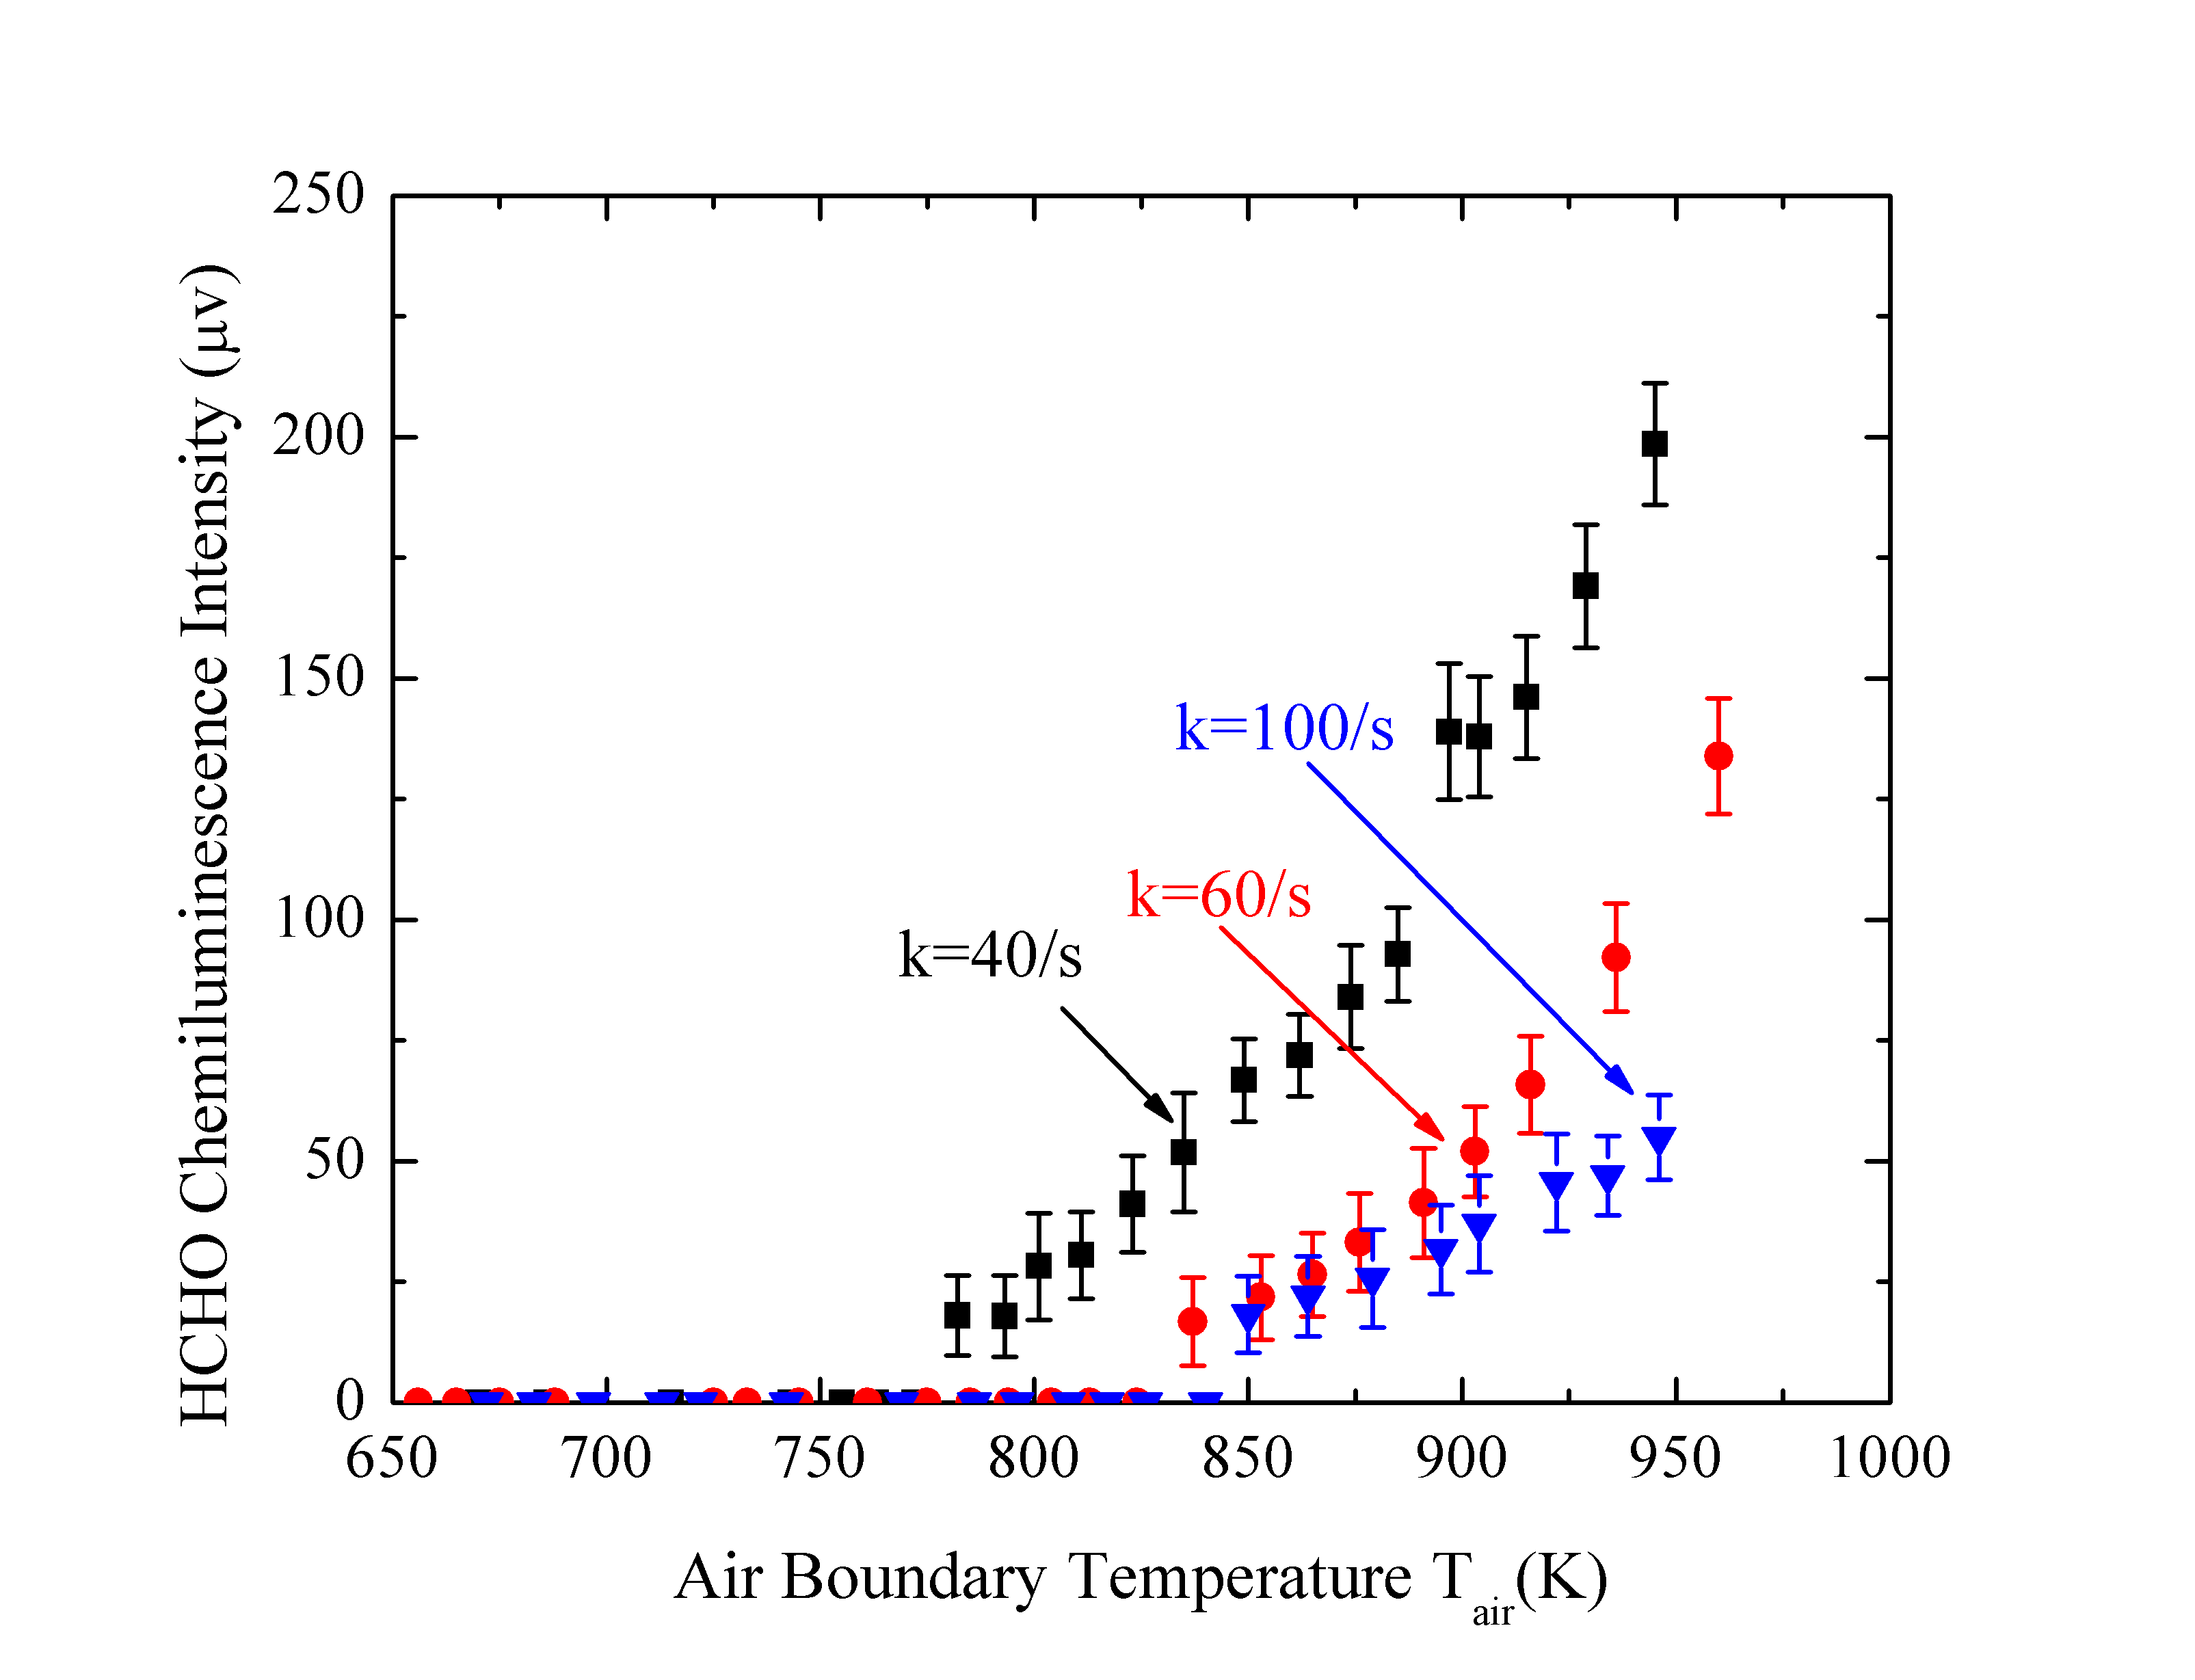
\includegraphics[width=0.6\textwidth]{PMT.png}
  \normalsize
  \vspace{-0.1in}
  \caption{HCHO chemiluminescence intensity at different air boundary temperatures under various strain rates.}
  \label{fig:PMT}
\end{figure}

The above experimental observations are further corroborated by the calculated results of the maximum formaldehyde (HCHO) mole fraction versus the air temperature for $30\%$ DME in nitrogen, for different strain rates.  Figure~\ref{fig:Scurve-SR} shows the calculated secondary S-curve characterized by the low-temperature chemistry.  It is seen that the upper branch solution, designating the state of the low-temperature flame, shows the same experimental trend of increasing HCHO concentration with increasing air temperature and decreasing strain rate.  We have therefore identified the presence of NTC-related chemical reactivity in the strongly transport-affected, nonpremixed counterflow.  The fact that this chemical reactivity is localized in a thin “flame” region is demonstrated in the next section.

\begin{figure}[t]
  \centering
  \scriptsize
  \vspace{-0.1in}
  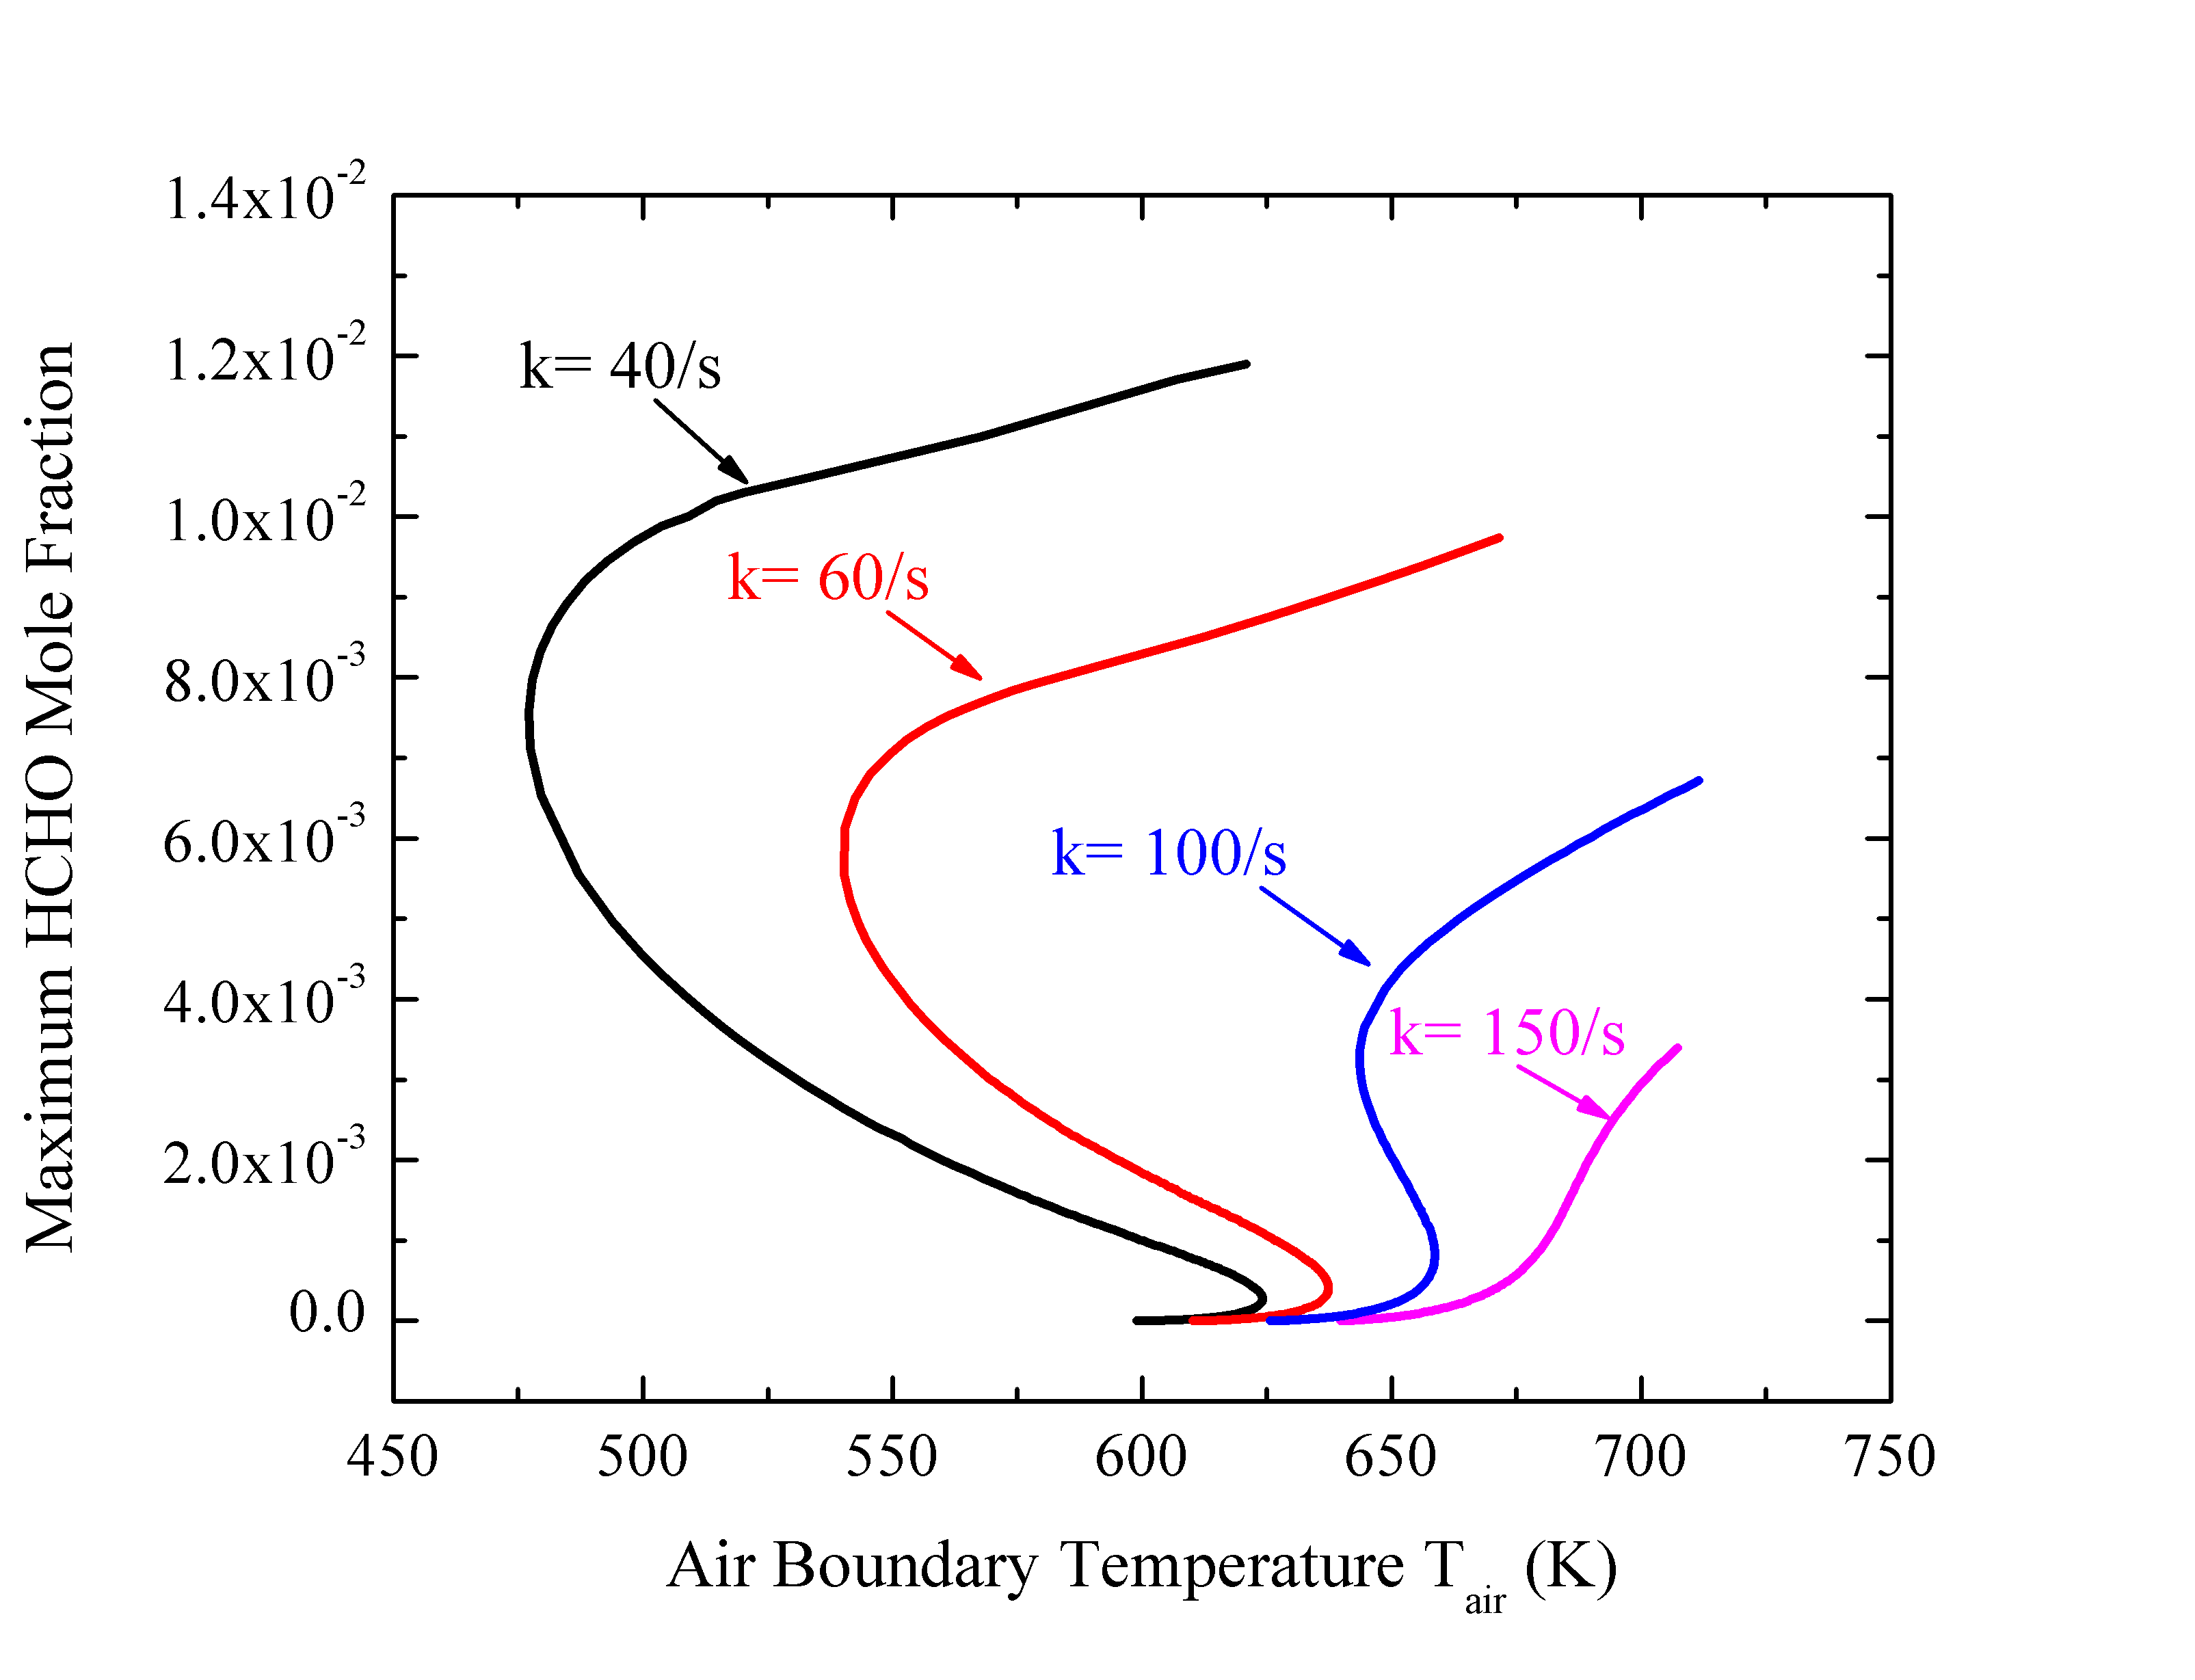
\includegraphics[width=0.6\textwidth]{Scurve-SR.png}
  \normalsize
  \vspace{-0.1in}
  \caption{Maximum HCHO mole fraction of $30\%$ DME at different air boundary temperatures under various strain rates.}
  \label{fig:Scurve-SR}
\end{figure}

\subsection{Determination of ignition temperature} \label{sec:4.2}

\begin{figure}[ht]
  \centering
  \scriptsize
  \vspace{0.1in}
  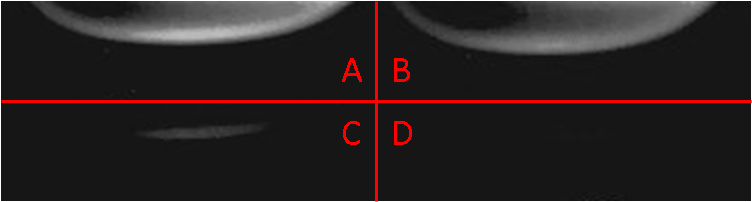
\includegraphics[width=0.5\textwidth]{IR.png}
  \normalsize
%  \vspace{-0.1in}
  \caption{A/B: Heated air/N$_2$ against DME counterflow IR images at ignition (atmospheric pressure, strain rate $60$ /s); C/D: Difference between A/B and B.}
  \label{fig:IR}
\end{figure}

We now proceed to detect the state of ignition of the NTC-flame, as identified by the lower turning points in Fig.~\ref{fig:Scurve-SR}.  Since the chemiluminescence intensity from the above experimentation is not strong enough to detect the low level of HCHO concentration at ignition, we have resorted to capturing the infrared radiation from the ignition process by using a highly sensitive infrared camera, FLIR SC640 (with the thermal sensitivity about $60$ mK at $303$ K), as shown on the right part of Fig.~\ref{fig:setup}.  The brightness of the IR images in Fig.~\ref{fig:IR} indicates the IR radiation intensity, with the bright color denoting higher radiation intensity than the dark color.  Since both the air/DME and N$_2$/DME flows now radiate infrared signals when heated due to the excitation of the vibrational modes of the gas molecules in the thermal mixing layer, the “background” N$_2$/DME signal needs to be subtracted out from the air/DME signal so as to isolate/identify the emission due to the low-temperature chemical reactivity.  Consequently, by gradually increasing the air boundary temperature, and by setting the IR radiation intensity of the N$_2$/DME flow as the reference state, the first appearance of an excess signal from the air/DME flow would indicate the onset of ignition.  In practice, when the air boundary temperature reaches the regime of interests, only $1$ K is increased each time at the air boundary before the flow becomes steady again.  It is fairly clear that at a certain temperature, which is defined as the ignition point, the signal from air/DME starts to exceed that of the reference state.  Such temperature measurements are repeatable within $\pm 2$ K.  A typical result is shown in Fig.~\ref{fig:IR}, in which the A and B panels are the raw IR signals for heated air and N$_2$ against DME, which are respectively reactive and nonreactive.  Panels C and D respectively show the residue signals of panels A and B after the background signal from panel B is subtracted; the null signal for D is obtained by default.  The temperature at which a discernable image of radiation is detected is then identified as that of ignition, as is the case for panels A/C, for the corresponding strain rate.

The localized nature of the IR radiation, shown in panel C, then also supports the notion that the chemical reactivity observed herein has the characteristic of a flame, in support of the interpretation of the chemiluminescence signal reported in the previous section.

Figure~\ref{fig:Ign-SR} shows the IR measurements of the low-temperature chemistry induced ignition, as determined through the above procedure, as a function of the strain rate.  The uncertainty bars account for those from the thermocouple radiation correction as well as reproducibility of the experimental measurements.  Due to the moderate flow field temperatures and the high sensitivity of the thermocouple, the uncertainty bars of the ignition temperatures are quite small.  These experimental values are then compared with those corresponding to the calculated lower, ignition turning points.  Figure~\ref{fig:Ign-SR} shows satisfactory agreement, with the average temperature difference being within $20$ K.

Sensitivity analysis was further performed for the state of ignition, as shown in Fig.~\ref{fig:Sen_SR}.  It is seen that the controlling chemistry is indeed the low tempearature chemistry, corresponding to the first stage ignition of the homogeneous autoignition process in the NTC-affect regime.  More specifically, the first two most important reactions that promote the low temperature chemistry induced ignition are the oxygen combination reaction: CH$_2$OCH$_2$O$_2$H+O$_2$ $\Leftrightarrow$ O$_2$CH$_2$OCH$_2$O$_2$H and the isomerization reaction: CH$_3$OCH$_2$O$_2$ $\Leftrightarrow$ CH$_2$OCH$_2$O$_2$H, while the most important retarding reaction is the $\beta$-scission reaction: CH$_2$OCH$_2$O$_2$H $\Leftrightarrow$ OH+$2$HCHO.  These two groups of reactions compete for the CH$_2$OCH$_2$O$_2$H radicals and as such function oppositely.

\begin{figure}[t]
  \centering
  \scriptsize
  \vspace{-0.1in}
  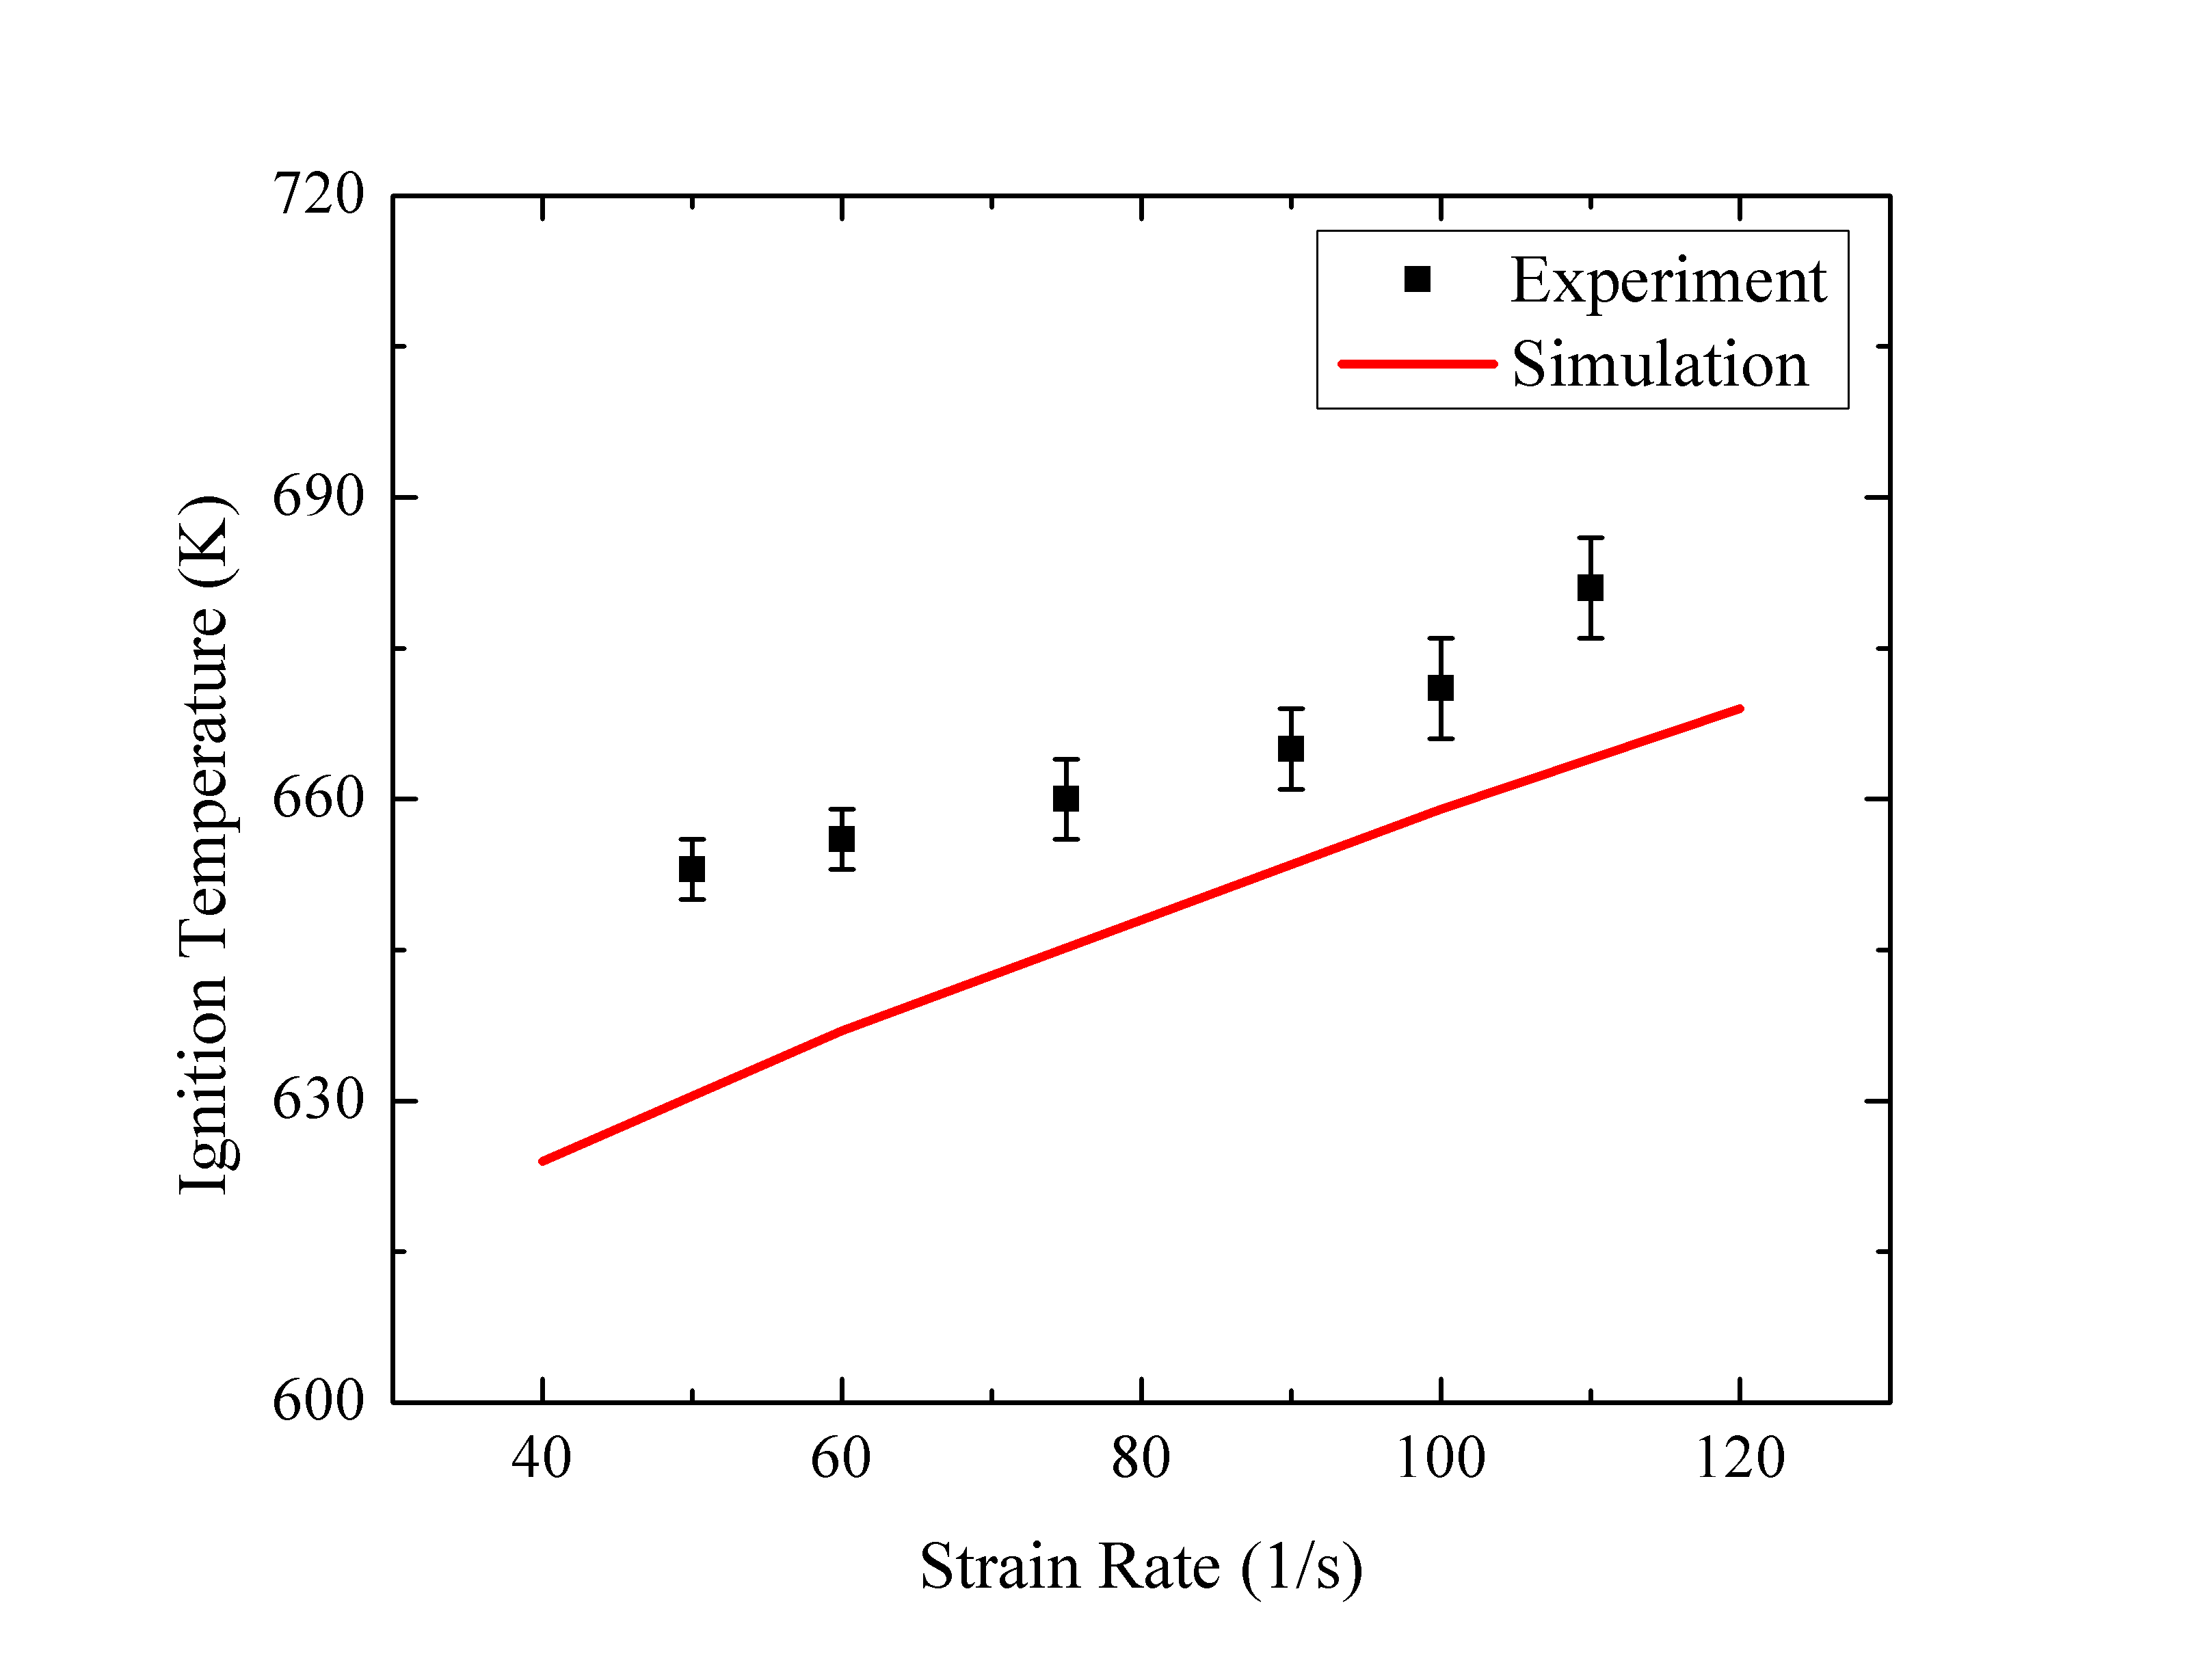
\includegraphics[width=0.6\textwidth]{Ign-SR.png}
  \normalsize
  \vspace{-0.1in}
  \caption{Calculated and observed ignition temperatures of $30\%$ DME under various strain rates.}
  \label{fig:Ign-SR}
\end{figure} 

\begin{figure}[t]
  \centering
  \scriptsize
  \vspace{-0.1in}
  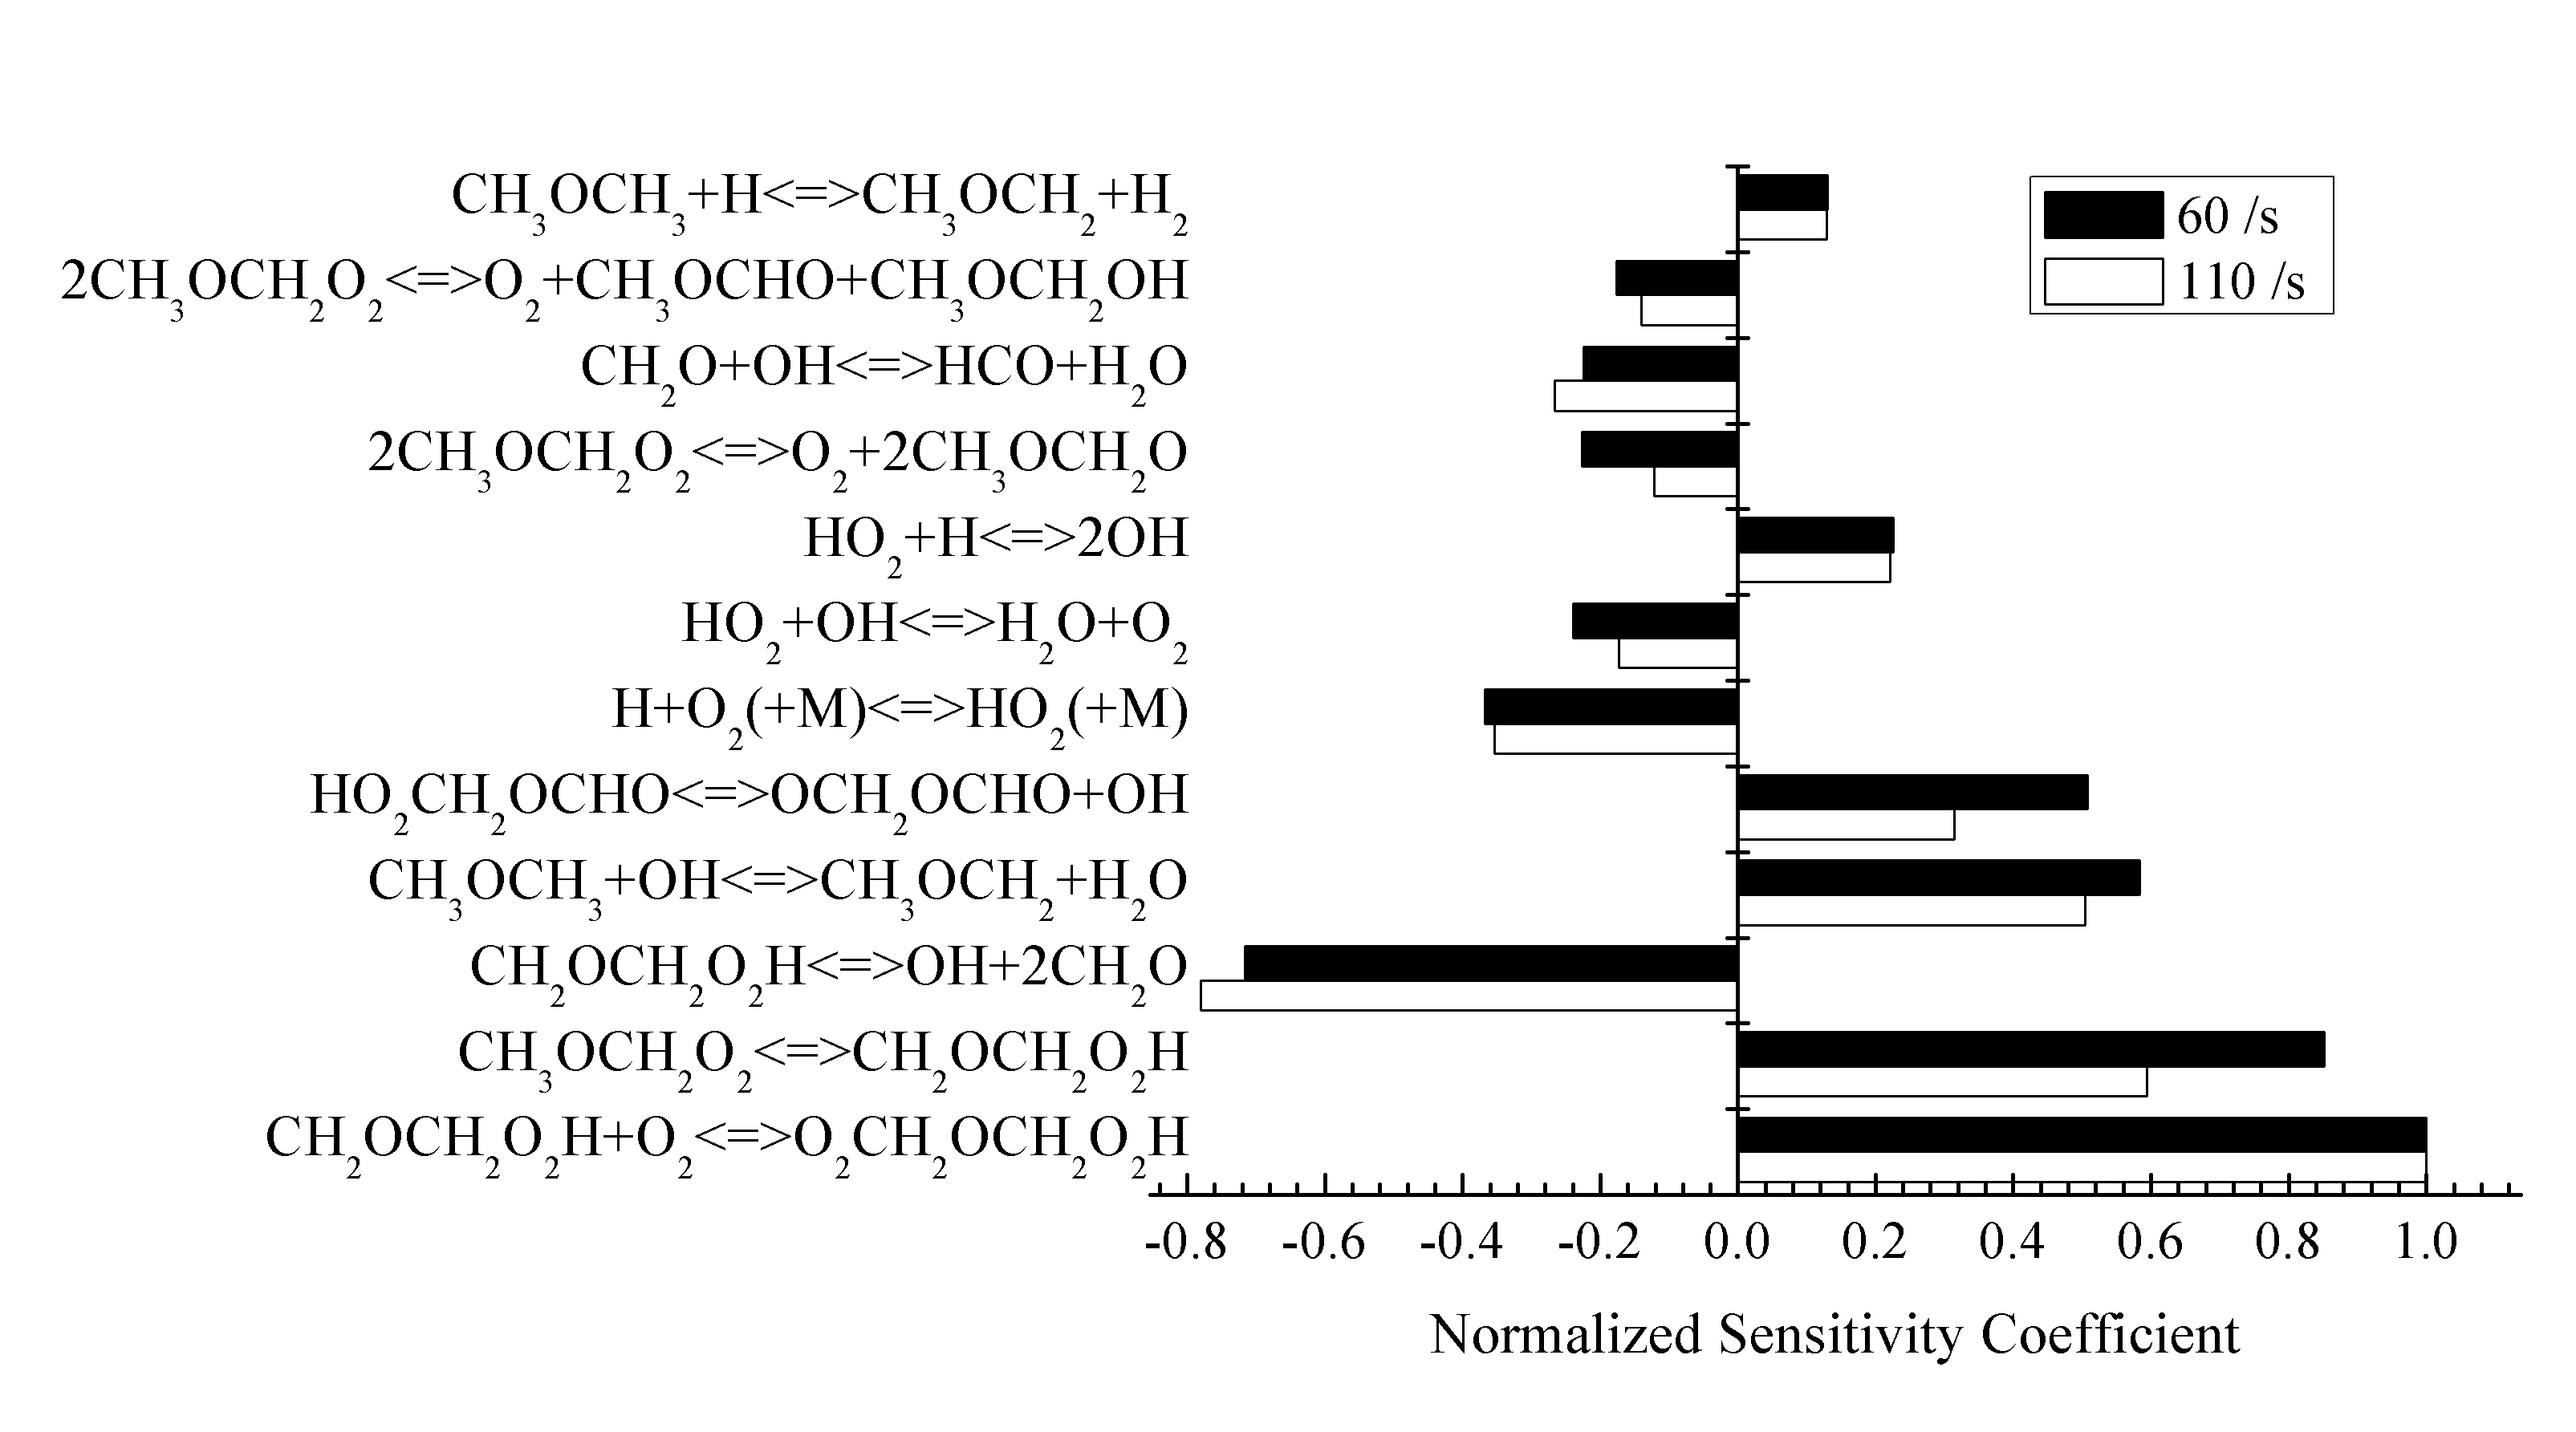
\includegraphics[width=0.7\textwidth]{Sen_SR.png}
  \normalsize
  \vspace{-0.1in}
  \caption{Sensitivity analysis on low and high strain rate cases: DME mole fraction is $30\%$.}
  \label{fig:Sen_SR}
\end{figure}

In addition to the effects of strain rate on the ignition temperature, we have also evaluated the effects of DME concentration, shown and compared with the simulation results in Fig.~\ref{fig:Ign-Con}.  The simulation result basically demonstrates the insensitive nature of the NTC-affected ignition temperature to the variation of the boundary DME concentrations over an extensive range of DME concentrations, under a fixed strain rate of $60$ /s.  The experimental results again show good agreement with the simulation results.  This effect corresponds to the insensitive nature of the equivalence ratio in the low-temperature chemistry, given the fact that the first-stage delay is insensitive to the equivalence ratio in the homogeneous autoignition process~\cite{zhao13}.  Sensitivity analysis corresponding to different boundary DME concentrations were also carried out, showing the same controlling chemistry as that of Fig.~\ref{fig:Sen_SR}.

\begin{figure}[t]
  \centering
  \scriptsize
  \vspace{-0.1in}
  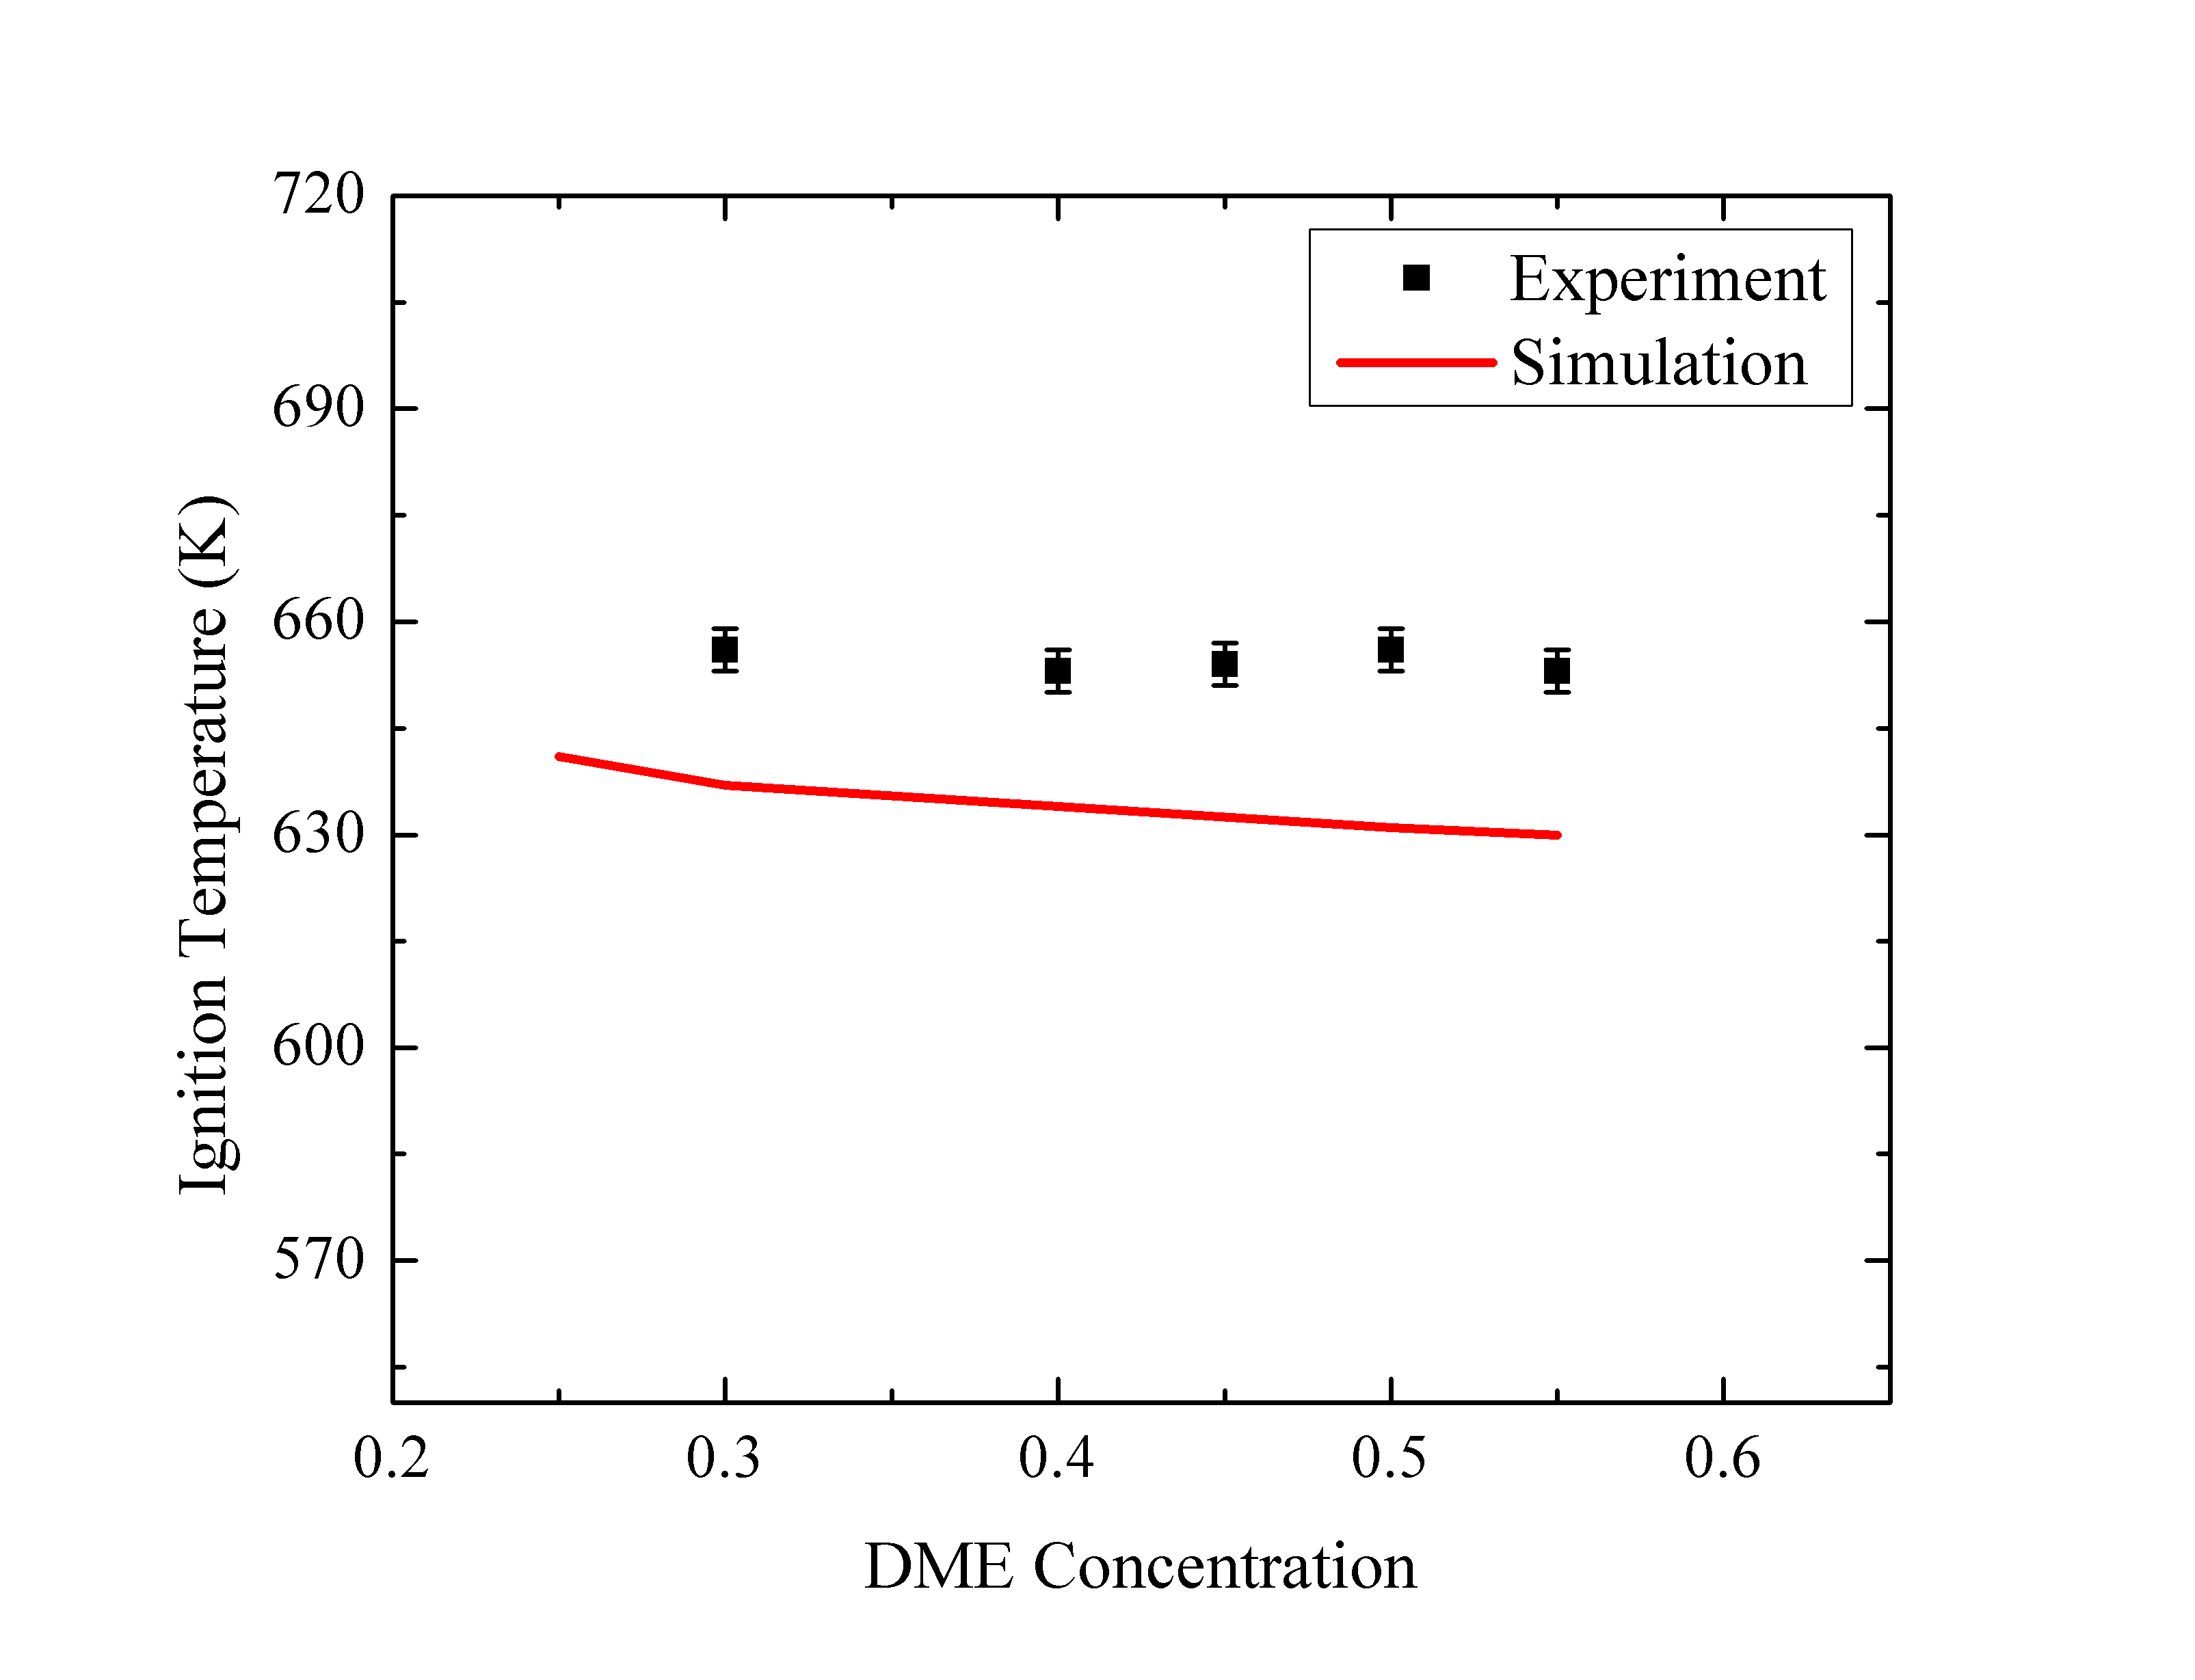
\includegraphics[width=0.6\textwidth]{Ign-Con.png}
  \normalsize
  \vspace{-0.1in}
  \caption{Ignition temperatures of various DME concentrations under the strain rate of $60$ /s.}
  \label{fig:Ign-Con}
\end{figure}


\section{Conclusions}        

Following our previous computational studies~\cite{law12,zhao13} that predicted the existence of low-temperature, NTC-affected, weakly burning diffusion flames in the counterflow, we have now successfully provided experimental substantiation of the existence of such flames.  In particular, the filtered PMT imaging demonstrated the presence of the signature HCHO chemiluminescence in the counterflow of heated air stream against nitrogen-diluted DME, while sensitive infrared imaging determined the corresponding ignition temperature.  Extensive experimentation then demonstrated that the low-temperature reactivity is enhanced with increasing air temperature, decreasing strain rate of the flow, and is insensitive to the DME concentrations.  Parallel computation substantiated the experimental results, and further corroborated the essential NTC chemistry governing the observed phenomena.

\section*{Acknowledgments}
This work was supported by the Combustion Energy Frontier Research Center, an Energy Frontier Research Center funded by the US Department of Energy, Office of Basic Energy Sciences under Award Number DE-SC0001198.

\section*{References}
\bibliographystyle{elsarticle-num-CNF}
\bibliography{NTC}

\renewcommand{\thefigure}{\arabic{figure}}
\renewcommand{\thetable}{\arabic{table}}

\end{document}

